
上一節的結果可能會有些沮喪。處理器非常複雜,需要處理很多問題才能以最高效率運行。這裡,我們從簡單的開始,看看處理器基本操作的速度。為此,我們將使用谷歌基準測試工具。下面是兩個數組簡單相加的基準測試:

\hspace*{\fill} \\ %插入空行
\noindent
\textbf{01\_superscalar.C}
\begin{lstlisting}[style=styleCXX]
#include "benchmark/benchmark.h"
void BM_add(benchmark::State& state) {
	srand(1);
	const unsigned int N = state.range(0);
	std::vector<unsigned long> v1(N), v2(N);
	for (size_t i = 0; i < N; ++i) {
		v1[i] = rand();
		v2[i] = rand();
	}
	unsigned long* p1 = v1.data();
	unsigned long* p2 = v2.data();
	for (auto _ : state) {
		unsigned long a1 = 0;
		for (size_t i = 0; i < N; ++i) {
			a1 += p1[i] + p2[i];
		}
		benchmark::DoNotOptimize(a1);
		benchmark::ClobberMemory();
	}
	state.SetItemsProcessed(N*state.iterations());
}
BENCHMARK(BM_add)->Arg(1<<22);
BENCHMARK_MAIN();
\end{lstlisting}

第一個例子,展示了基準的所有細節,包括輸入的生成。大多數操作的速度並不依賴於操作數的值,這裡使用隨機輸入,這樣在處理對輸入敏感的操作時就不用擔心了。雖然將值存儲在數組中,但我們不想測試數組索引的速度:編譯器肯定會優化表達式\texttt{v1[i]},以生成與\texttt{p1[i]}完全相同的代碼,但為什麼要冒這個險呢?將盡可能多的不重要的細節排除在外,直到剩下最基本的問題。內存中有兩個數組,我們想對數組的每個元素進行一些計算。

另一方面,必須考慮不需要的編譯器優化的可能。編譯器可能會發現整個程序只是一個非常長,且什麼都不做的過程(至少就C++標準而言是這樣的),並通過優化掉大塊的代碼,給出一個更快的方法來做同樣的事情。編譯器的方向是不要優化掉計算的結果,並假定內存的狀態可以在基準迭代之間進行修改,這也會阻止此類優化。另外,將變量\texttt{a1}聲明為\texttt{volatile}肯定會阻止大多數不應該的優化。反過來,它也會阻止編譯器優化循環,這不是我們想要的結果。我們想看到CPU如何高效地處理兩個數組,也就是如何生成最高效的代碼。我們只是不想讓編譯器發現基準循環的第一次迭代與第二次迭代完全相同。

微基準測試的一個不尋常的應用。有一小段代碼,我們想知道它有多快,以及如何使它更快。我們使用微基準來瞭解處理器的性能,通過對代碼進行裁剪,帶給一些啟發。

編譯基準測試時,應該打開優化選項。運行基準測試將產生如下的結果(當然確切的數字取決於CPU):

%\hspace*{\fill} \\ %插入空行
\begin{center}
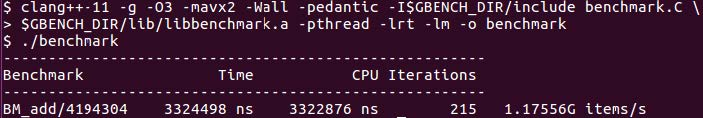
\includegraphics[width=0.9\textwidth]{content/1/chapter3/images/2.jpg}\\
圖 3.2
\end{center}

目前,我們還不能從這個實驗中得出什麼結論(除了現代CPU速度的確快)。CPU可以在不到1納秒的時間內將兩個數字相加。如果對此感到好奇,可以探索一下其他運算:減法和乘法所花費的時間與加法相同,而整數除法則相當緩慢(比加法慢三到四倍)。

為了分析代碼的性能,必須按照處理器的方式來進行。兩個輸入數組存儲在內存中,但是加法或乘法操作是在存儲在寄存器中的值之間執行的(對於某些操作,可能是在寄存器和內存位置之間)。這就是處理器如何一步步地對循環進行迭代。迭代開始時,索引變量\texttt{i}在一個CPU寄存器中,對應的兩個數組元素\texttt{v1[i]}和\texttt{v2[i]}在內存中:

%\hspace*{\fill} \\ %插入空行
\begin{center}
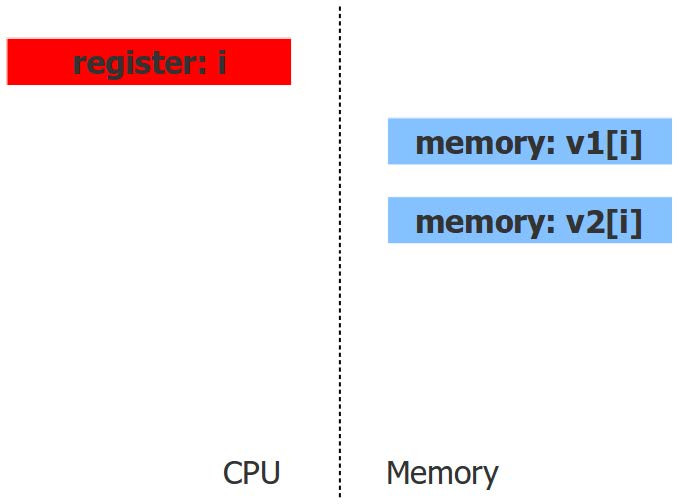
\includegraphics[width=0.6\textwidth]{content/1/chapter3/images/3.jpg}\\
圖 3.3
\end{center}

做計算之前,必須將輸入移到寄存器中。必須為每個輸入分配一個寄存器,併為結果分配一個寄存器。在給定的循環迭代中,第一個指令會把一個輸入加載到寄存器中:

%\hspace*{\fill} \\ %插入空行
\begin{center}
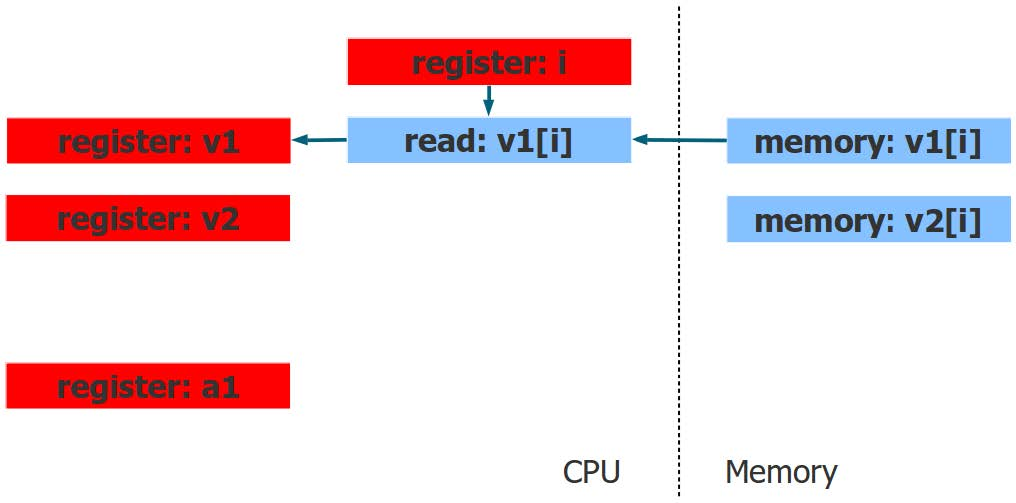
\includegraphics[width=0.7\textwidth]{content/1/chapter3/images/4.jpg}\\
圖3.4 - 第i次迭代:第一個指令後的處理器狀態
\end{center}

read(或load)指令使用內存中包含索引\texttt{i}和數組\texttt{v1}位置的寄存器來訪問值\texttt{v1[i]},並將其複製到寄存器中。下一條指令以相同的方式來加載第二個輸入:

%\hspace*{\fill} \\ %插入空行
\begin{center}
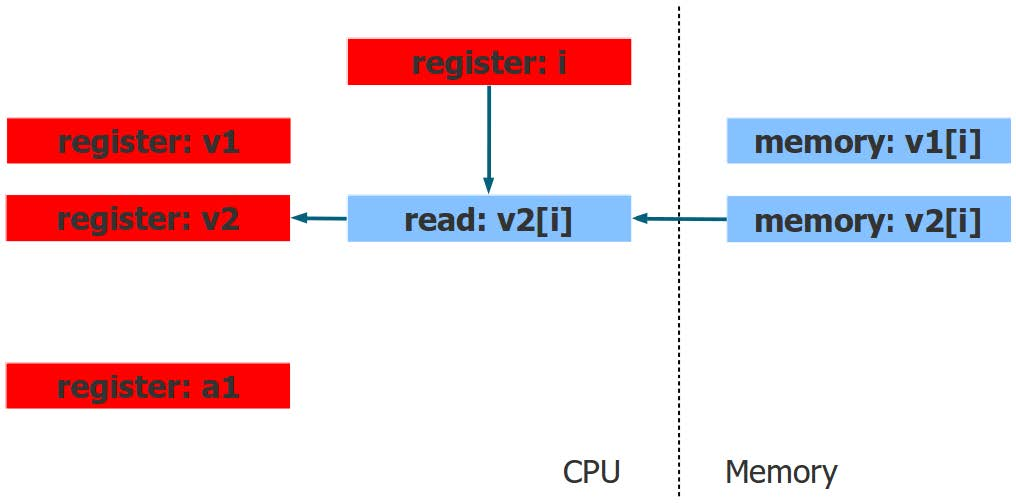
\includegraphics[width=0.7\textwidth]{content/1/chapter3/images/5.jpg}\\
圖3.5 - 第i次迭代:第2條指令後的處理器狀態
\end{center}

現在可以進行加法或乘法運算了:

%\hspace*{\fill} \\ %插入空行
\begin{center}
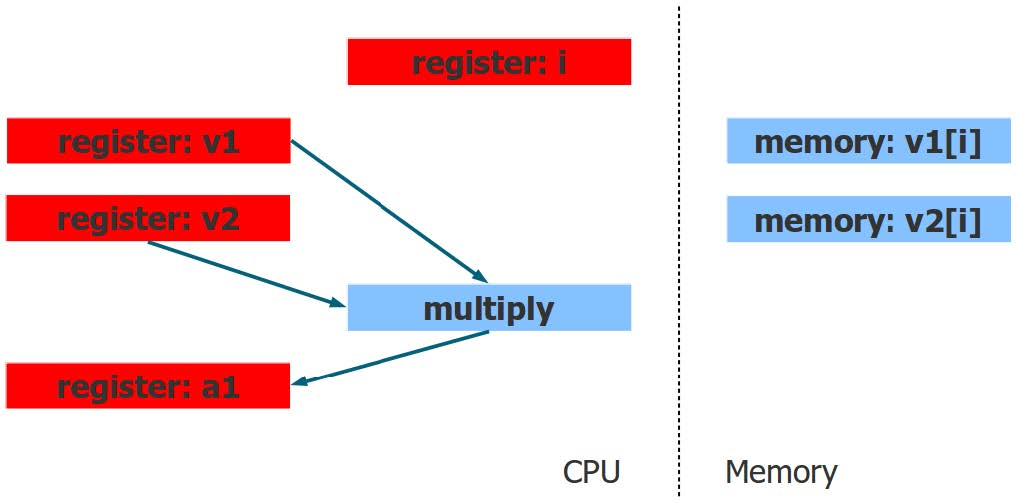
\includegraphics[width=0.7\textwidth]{content/1/chapter3/images/6.jpg}\\
圖3.6 -第i次循環迭代結束時的處理器狀態
\end{center}

這行簡單的代碼在轉換成硬件指令後,就產生了所有這些操作(加上進入下一次循環迭代所需的操作):

\begin{lstlisting}[style=styleCXX]
a1 += p1[i] + p2[i];
\end{lstlisting}

從效率的角度來看,我們只關注最後一步。CPU可以在一納秒內把兩個數字相加或相乘,這已經很好了,但還能做得更好嗎?許多晶體管都致力於處理和執行指令,所以它們能處理更多的東西。讓我們嘗試對相同的值做兩個操作,而不是一個:

\hspace*{\fill} \\ %插入空行
\noindent
\textbf{01\_superscalar.C}
\begin{lstlisting}[style=styleCXX]
void BM_add_multiply(benchmark::State& state) {
	… prepare data …
	for (auto _ : state) {
		unsigned long a1 = 0, a2 = 0;
		for (size_t i = 0; i < N; ++i) {
			a1 += p1[i] + p2[i];
			a2 += p1[i] * p2[i];
		}
		benchmark::DoNotOptimize(a1);
		benchmark::DoNotOptimize(a2);
		benchmark::ClobberMemory();
	}
	state.SetItemsProcessed(N*state.iterations());
}
\end{lstlisting}

如果加法和乘法都需要1納秒,那麼兩者都需要多長時間?基準測試給了我們答案:

%\hspace*{\fill} \\ %插入空行
\begin{center}
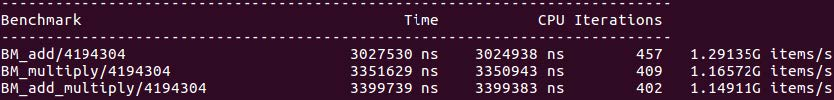
\includegraphics[width=0.9\textwidth]{content/1/chapter3/images/7.jpg}\\
圖3.7 - 一條指令和兩條指令的基準測試
\end{center}

令人驚訝的是,這裡一加一,居然等於一。我們可以在一次迭代中添加更多的指令:

\begin{lstlisting}[style=styleCXX]
for (size_t i = 0; i < N; ++i) {
	a1 += p1[i] + p2[i];
	a2 += p1[i] * p2[i];
	a3 += p1[i] << 2;
	a4 += p2[i] – p1[i];
}
\end{lstlisting}

每次迭代的時間仍然相同(基準測量的精度範圍內略有差異):

%\hspace*{\fill} \\ %插入空行
\begin{center}
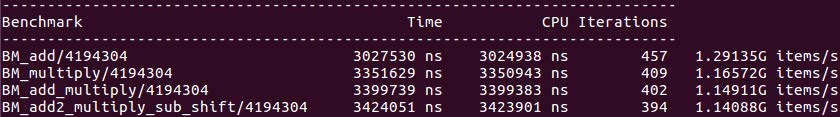
\includegraphics[width=0.9\textwidth]{content/1/chapter3/images/8.jpg}\\
圖3.8 - 每次迭代最多有四條指令循環的基準測試結果
\end{center}

我們認為處理器每次只執行一條指令的觀點需要修正了:

\hspace*{\fill} \\ %插入空行
\begin{center}
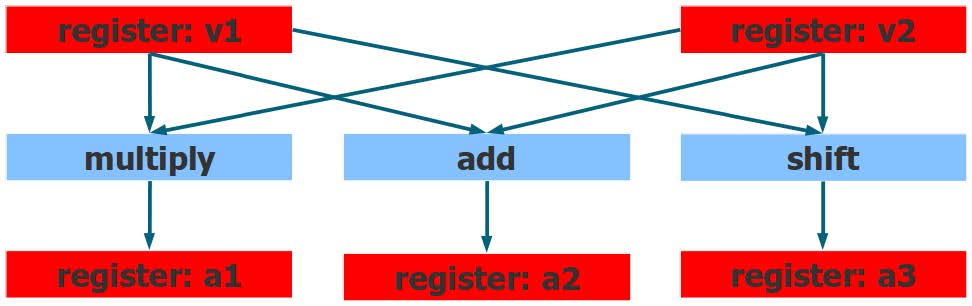
\includegraphics[width=0.9\textwidth]{content/1/chapter3/images/9.jpg}\\
圖3.9 - 處理器在一次執行多個操作
\end{center}

只要操作數在寄存器中了,處理器就可以同時執行多個操作,這就是所謂的\textbf{指令級並行(ILP)}。當然,可以執行多少操作是有限制的,處理器能夠執行整數的計算單元是有限的。儘管如此,通過在一次迭代中添加越來越多的指令,嘗試將CPU推向極限是有指導意義的:

\begin{lstlisting}[style=styleCXX]
for (size_t i = 0; i < N; ++i) {
	a1 += p1[i] + p2[i];
	a2 += p1[i] * p2[i];
	a3 += p1[i] << 2;
	a4 += p2[i] – p1[i];
	a5 += (p2[i] << 1)*p2[i];
	a6 += (p2[i] - 3)*p1[i];
}
\end{lstlisting}

當然,處理器可以執行的指令數量取決於CPU和指令,但與單個乘法運算相比,前面的循環速度明顯出現了下降,至少在我使用的機器上是這樣:

%\hspace*{\fill} \\ %插入空行
\begin{center}
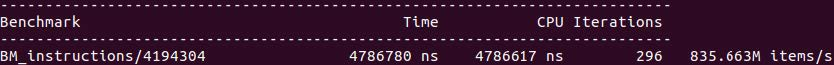
\includegraphics[width=0.9\textwidth]{content/1/chapter3/images/10.jpg}\\
圖3.10 - 每迭代8條指令的基準測試結果
\end{center}

就硬件利用率而言,可以看到最初的代碼是多麼低效。CPU顯然可以在每次迭代中執行5到7個不同的操作,因此單個乘法甚至用不到其能力的四分之一。事實上,現代處理器的能力更令人吃驚。除了我們一直在試驗的整數計算單元外,還有單獨的浮點硬件,可以在雙精度或浮點值上執行指令,以及同時執行MMX、SSE、AVX和其他專門指令的向量處理單元!

\subsubsubsection{3.3.1\hspace{0.2cm}可視化的指令級並行}

目前,我們關於CPU並行執行多條指令能力的結論還是基於間接證據。如果能直接確認這就是事實,那就太好了。我們可以從\textbf{機器碼分析器(MCA)}得到這樣的確認,它是LLVM工具鏈的一部分。分析器將彙編代碼作為輸入,並獲得關於指令如何執行、延遲和瓶頸是什麼等信息。我們不打算在這裡學習這個高級工具的功能(詳細信息請參閱項目主頁,\url{https://llvm.org/docs/CommandGuide/llvm-mca.html})。現在,可以使用它來查看CPU如何執行操作的。

第一步是用分析器標記註釋代碼,選擇要分析的代碼段:

\begin{lstlisting}[style=styleCXX]
#define MCA_START __asm volatile("# LLVM-MCA-BEGIN");
#define MCA_END __asm volatile("# LLVM-MCA-END");
…
for (size_t i = 0; i < N; ++i) {
MCA_START
	a1 += p1[i] + p2[i];
MCA_END
}
\end{lstlisting}

不必為分析器標記使用\texttt{\#define},但記住這些命令比記住精確的彙編語法要容易(可以保存\texttt{\#define}在頭文件中,並在需要時包含)。為什麼只標記循環的主體,而不是整個循環呢?分析器實際上假設所選的代碼片段在一個循環中運行,並將其重複若干次迭代(默認情況下為10次)。可以嘗試為分析標記整個循環。但根據編譯器的優化,這可能會使分析器感到困惑(這是一個強大的工具,但不容易使用)。

現在運行分析器:

%\hspace*{\fill} \\ %插入空行
\begin{center}
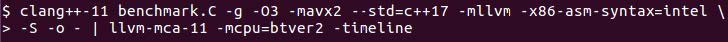
\includegraphics[width=0.9\textwidth]{content/1/chapter3/images/11.jpg}\\
圖 3.11
\end{center}

我們不是把代碼編譯成可執行文件,而是用Intel語法生成彙編輸出(\texttt{-S})。輸出輸送到分析器,在分析器可以報告結果的許多方式中,我們選擇了時間軸輸出。時間軸視圖顯示每條指令在執行過程中的移動。我們分析兩個代碼片段,一個使用單個操作(加法或乘法),另一個使用兩個操作。以下是迭代的時間線,只有一次乘法(我們已經刪除了時間線中間的所有行):

%\hspace*{\fill} \\ %插入空行
\begin{center}
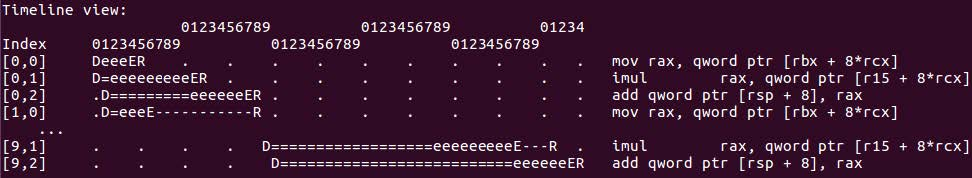
\includegraphics[width=0.9\textwidth]{content/1/chapter3/images/12.jpg}\\
圖 3.12
\end{center}

橫軸是時的週期,該分析模擬運行選定的代碼片段十次迭代,每條指令都由其在代碼中的序號和迭代索引來標識,因此第一次迭代的第一條指令的索引為[0,0],最後一條指令的索引為[9,2]。最後一條指令也是第十次迭代的第三條指令(每次迭代只有三條指令)。根據時間軸,整個過程需要55個週期。

從內存中讀取\texttt{p1[i]}和\texttt{p2[i]},對其進行操作:

\begin{lstlisting}[style=styleCXX]
#define MCA_START __asm volatile("# LLVM-MCA-BEGIN");
#define MCA_END __asm volatile("# LLVM-MCA-END");
…
for (size_t i = 0; i < N; ++i) {
MCA_START
	a1 += p1[i] + p2[i];
	a2 += p1[i] * p2[i];
MCA_END
}
\end{lstlisting}

讓我們看看每個迭代有兩個操作的時間軸,一個加法和一個乘法:

%\hspace*{\fill} \\ %插入空行
\begin{center}
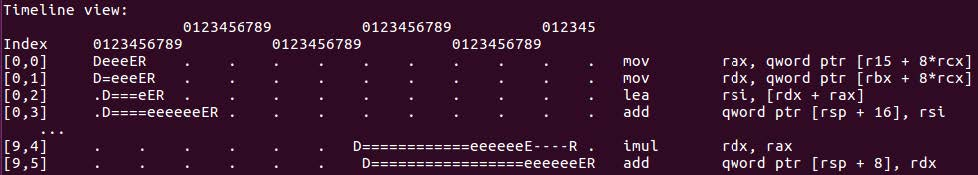
\includegraphics[width=0.9\textwidth]{content/1/chapter3/images/13.jpg}\\
圖 3.13
\end{center}

現在執行的指令更多了,每次迭代有6條指令(最後一條指令有索引[9,5])。時間軸的持續時間只增加了一個週期。圖3.12中,時間軸結束於第54週期,而在圖3.13中,結束於第55週期。正如我們所懷疑的那樣,處理器在同樣長的時間內執行了兩倍的指令。

可能還注意到,對於目前為止的所有基準測試,我們都增加了對相同輸入值執行的操作的數量(添加、減去、乘以等)。就運行時而言,這些額外的操作是免費的(在一定程度上),這是非常重要的經驗:當在寄存器中有了一些值,在相同的值上加法計算可能不會降低任何性能,除非程序已經非常高效,並且將硬件壓到了極限。遺憾的是,實驗和結論的實用價值有限。所有計算在同一時間只執行少量輸入,下一次迭代使用自己的輸入,並且可以在相同的輸入上找到一些更有用的計算,這種情況發生的頻率有多高呢?也不是沒有,但很少。擴展我們對CPU計算能力的簡單演示將會遇到一個或多個難題,首先就是數據依賴。循環的順序迭代通常不獨立,可能每個迭代都需要一些來自前面迭代的數據。下一節將探討這種情況。

















